\section{Experiment and Result}


\subsubsection{Bi-directional LSTM}
\subsubsection{Batch Normalization}

\subsection{Multi-View Lip-Reading}
\subsubsection{Visual Model Architecture}
\subsubsection{Data-Augmentation}


\begin{table}[h]
\centering
    \begin{tabular}{ccc|cccccc}
        \multicolumn{3}{c|}{Architecture} &%
        \multicolumn{6}{c}{View}\\ \hline
        Visual  & Temporal & Classifier &%
        0& 30 & 45 & 60 & 90 & multi\\\hline
        %
        \multirow{2}{*}{CNN-org}%
        & LSTM & \multirow{2}{*}{SVM} &%
        & & & & &\\
        & biLSTM & &%
        & & & & &\\
        \multirow{2}{*}{Alex}%
        & LSTM & \multirow{2}{*}{SVM} &%
        & & & & &\\
        & biLSTM & &%
        & & & & &\\
        \multirow{2}{*}{Key}%
        & LSTM & \multirow{2}{*}{SVM} &%
        & & & & &\\
        & biLSTM & &%
        & & & & &\\
        \multirow{2}{*}{Opti}%
        & LSTM & \multirow{2}{*}{SVM} &%
        & & & & &\\
        & biLSTM & &%
        & & & & &\\
    \end{tabular}
    \caption{Results obtained with a single visual, temporal and classifier is used}
    \label{tab:resDiffArch}
\end{table}

\begin{table}[h]
\centering
    \begin{tabular}{ccc|cccccc}
        \multicolumn{3}{c|}{Architecture} &%
        \multicolumn{6}{c}{View}\\ \hline
        Visual  & Temporal & Classifier &%
        0& 30 & 45 & 60 & 90 & multi\\\hline
        %
        \multirow{2}{*}{CNN+key}%
        & LSTM & \multirow{2}{*}{SVM} &%
        & & & & &\\
        & biLSTM & &%
        & & & & &\\
        \multirow{2}{*}{CNN+opti}%
        & LSTM & \multirow{2}{*}{SVM} &%
        & & & & &\\
        & biLSTM & &%
        & & & & &\\
        \multirow{2}{*}{Alex+key}%
        & LSTM & \multirow{2}{*}{SVM} &%
        & & & & &\\
        & biLSTM & &%
        & & & & &\\
        \multirow{2}{*}{Alex+opti}%
        & LSTM & \multirow{2}{*}{SVM} &%
        & & & & &\\
        & biLSTM & &%
        & & & & &\\
    \end{tabular}
    \caption{Results obtained when multiple visual models is combined}
    \label{tab:resDiffArch}
\end{table}


\subsection{Single-view Lip-Reading}

\begin{figure}[h]
	\centering
	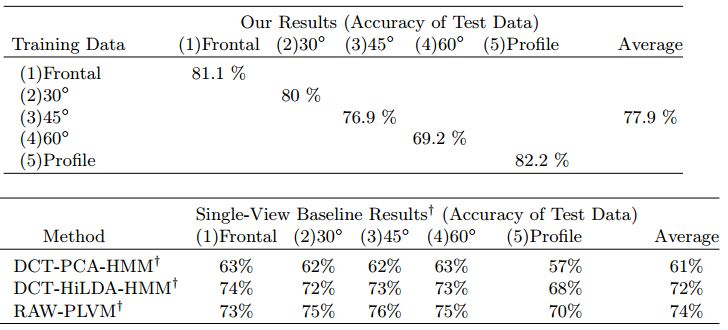
\includegraphics[width=\columnwidth]{fig/s1.jpg}
	\caption{Single-view test accuray of word phrases.}
	\label{fig:s1}
\end{figure}
Fig \ref{fig:s1} shows the accuracy result of single - view on word phrase test data. The results are similar to the one presented in \cite{Lee}. We have best accuracy on Profile view.

\begin{figure}[h]
	\centering
	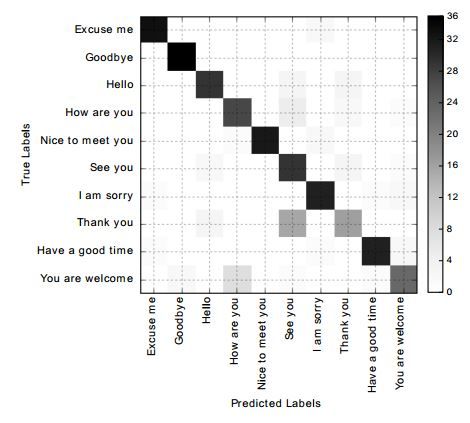
\includegraphics[width=\columnwidth]{fig/s2.jpg}
	\caption{Confusion matrix of best of Single Views}
	\label{fig:s2}
\end{figure}
Fig \ref{fig:s2} is Confusion matrix of profile view, which is the best in single view test accuracy. The x-axis is prediction classes and the y-axis is true classes.
We can see that 'Thank you' and 'See you' is the most confusing word phrase.


\subsection{Cross-view Lip-Reading}
In Cross view experiment, we conduct it as two seperate stages. At first stage, as we refer it to 'Cross View(CV)', we train 5 total view data all together simultaneously and test each view seperately.  In this approach, we get the
average accuracy 82.6\%, and all of the results are better than preliminary results.
 At Second stage, we call this stage as "Cross-view2(CV2)", and here, we finetune the first stage result to a certain view and also test with the certain view. Here, we can see slightly better performance on each view and also on average compare to CV.
  
\begin{figure}[h]
	\centering
	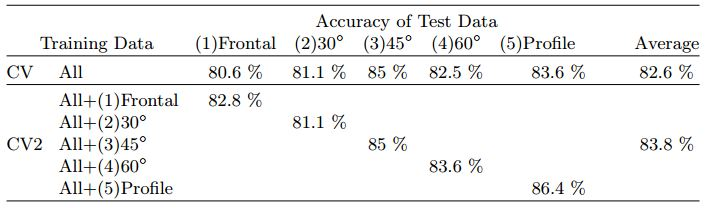
\includegraphics[width=\columnwidth]{fig/c1.jpg}
	\caption{Cross-view test accuracy. CV : Cross View, CV2 : Cross View 2}
	\label{fig:c1}
\end{figure}
In CV, Profile view shows the best performance(83.6\%), and in CV2, 60-degree view shows the best performance on total Cross view experiment.

\begin{figure}[h]
	\centering
	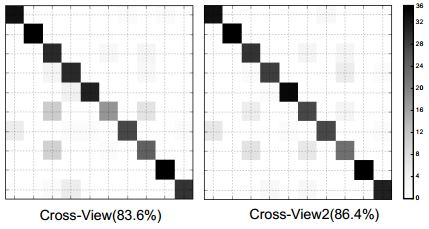
\includegraphics[width=\columnwidth]{fig/c2.jpg}
	\caption{Confusion matrices of best of  Cross Views}
	\label{fig:c2}
\end{figure}
The confusion matrices of test accuracies of profile view(CV) and 60-degree view (CV2). The axis lable share the same label in fig \ref{fig:s2}. It shows that
a gradual improvement from single-view to cross-view.  

\subsection{Multi-view Lip-Reading}
In Multi-view experiment, we conduct slightly different type of architecture as inputs are five times larger then single or cross view experimetn. Here, we conduct Merge Image method as this method of multi-view is best in our previous paper.

\subsubsection*{Merge Images}
\begin{figure}[h]
	\centering
	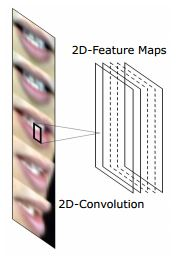
\includegraphics[width=0.4\columnwidth]{fig/mi.jpg}
	\caption{Merge Image model architencture for the multi-view setting}
	\label{fig:mi}
\end{figure}
As shown in fig \ref{fig:mi}, we append five images from the different
view at the same time into a single image as an input of the visual model. In this
architecture, we expect to learn all the five view feature by 2D-CNN. While out
of our experiment, a more elaborate configuration is that all five images avoid
convolving each other along the edges.

Despite it has more feature (give times more inputs), the result is worse than cross-view.
Fig \ref{fig:summary} shows the summary of all experiment through this paper.
\begin{figure}[h]
	\centering
	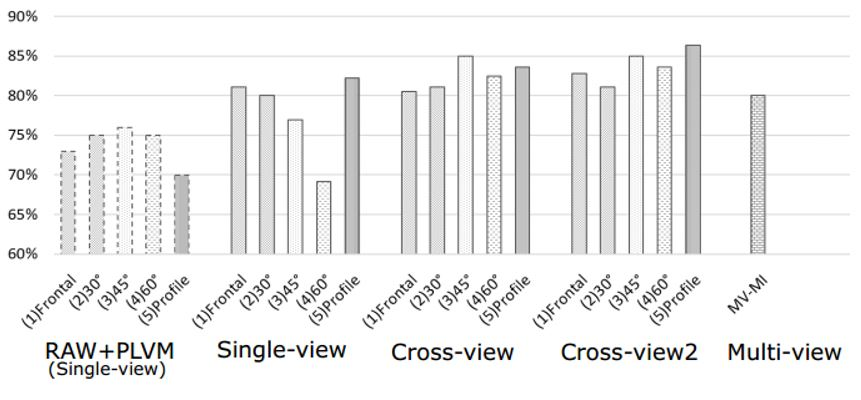
\includegraphics[width=\columnwidth]{fig/summary.jpg}
	\caption{The summary of the accuraciese. MV-MI is refers to Merge Images.}
	\label{fig:summary}
\end{figure}
